% Copyright 2019 Clara Eleonore Pavillet

% Author: Clara Eleonore Pavillet
% Description: This is an unofficial Oxford University Beamer Template I made from scratch. Feel free to use it, modify it, share it.
% Version: 1.0

\documentclass{beamer}
% Load Packages
\usepackage[utf8]{inputenc}
\usepackage{xcolor}
\usepackage{tikz}
\usetikzlibrary{positioning,calc}
\usepackage{graphicx}
\usepackage{hyperref}
\usepackage{amsmath}
\usepackage{listings}
\usepackage{fontawesome}
\usepackage{bm}

% Define Commands
\newcommand*{\ClipSep}{0.06cm} %To adjust footer logo
\newcommand{\E}{\mathrm{e}\,} %\def\I{e} % used to defined e for exp(x), see later what it should be
\newcommand{\ud}{\mathrm{d}}
\lstset{numbers=left, numberstyle=\tiny, stepnumber=1,firstnumber=1,breaklines=true,
    numbersep=5pt,language=Python,
    stringstyle=\ttfamily,
    basicstyle=\footnotesize, 
    showstringspaces=false
}

\usetheme{oxonian}

\title{Continual Lifelong Learning}
\titlegraphic{
\includegraphics[width=2cm]{Theme/Logos/OxfordLogoV1.png}}
\author{Jonas Wildberger}
\institute{University of Oxford}
\date{} %\today
\bibliographystyle{alpha}

\begin{document}

{\setbeamertemplate{footline}{} 
\frame{\titlepage}}

\section*{Outline}\begin{frame}{Outline}\tableofcontents\end{frame}

\section{Problem Description}
    \begin{frame}[plain]
        \vfill
      \centering
      \begin{beamercolorbox}[sep=8pt,center,shadow=true,rounded=true]{title}
        \usebeamerfont{title}\insertsectionhead\par%
        \color{oxfordblue}\noindent\rule{10cm}{1pt} \\
       
      \end{beamercolorbox}
      \vfill
  \end{frame}


\subsection{Machine vs. Human learning}
\begin{frame}{Machine vs. Human learning}
\begin{itemize}
	\item<1-> State-of-the art ANNs rival human performance in a variety of domain-specific tasks
	
	\item<2-> Inspired by human learning, yet substantially different
	\begin{itemize}
		\item<2-> Machine: Parameters used statically on new data
		\item<2-> Human: On-the-fly update of memories and beliefs
	\end{itemize}
	\item<3-> Necessity to retrain on entire dataset to avoid overfitting and catastrophic forgetting
\end{itemize}

\begin{center}
	\visible<4->{How do we enable learning in an online fashion for ANNs?}
\end{center}
\end{frame}

\subsection{Catastophic Forgetting}
\begin{frame}{Catastrophic Forgetting I}
	\begin{itemize}
		\item<1-> Performance on previous task catastrophically deteriorates when new task is learned
		\item<2-> Stability vs. Plasticity	
		\item<3-> Presumably caused by static weights
\end{itemize}
\begin{center}
	\visible<4->{Problem: Minimise total loss function without access to loss function of previous tasks}
\end{center}
\end{frame}

\begin{frame}{Catastrophic Forgetting II}
	\begin{figure}
	
	\centering
	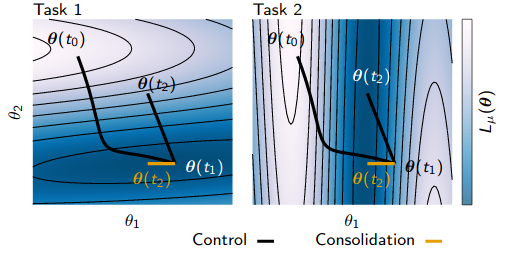
\includegraphics[width=0.8\textwidth]{ML1}
	\caption{Illustration of Catastrophic Forgetting \cite{zenke2017continual}}
\end{figure}
\end{frame}
\subsection{Overcoming Catastrophic Forgetting}

\begin{frame}{Overcoming Catastrophic Forgetting I}
\begin{enumerate}
	\item<1-> Architectural approach
	\begin{itemize}
		\item<1-> Alter architecture of network, e.g. freezing weights, changing learning rate for layers shared with original task, feature augmentation
	\end{itemize}
	\item<2-> Functional approach
	\begin{itemize}
		\item Add regularisation term that penalises changes in input-output function, i.e. predictions are similar across tasks
		\item Computationally expensive: For every new data point, compute forward pass through old task's network
		
	\end{itemize}


\end{enumerate}
\end{frame}
\begin{frame}{Overcoming Catastrophic Forgetting II}
	\begin{enumerate}
		\item[3.] Structural approach
		\begin{itemize}
			\item Penalties on the parameters s.t. they remain close to values for old task
			\item Mimic complexity of biological synapses
			\item Retain task relevant information and measure of importance
		\end{itemize} 
	\end{enumerate}
\end{frame}





\section{Elastic Weight Consolidation}
    \begin{frame}[plain]
        \vfill
      \centering
      \begin{beamercolorbox}[sep=8pt,center,shadow=true,rounded=true]{title}
        \usebeamerfont{title}\insertsectionhead\par%
        \color{oxfordblue}\noindent\rule{10cm}{1pt} 
        
      \end{beamercolorbox}
      \vfill
  \end{frame}
  
%\subsection{Example}
\begin{frame}{Bayesian Foundation}

Let $\mathcal D_A, \mathcal D_B$ be two \textcolor{oxfordblue}{independent} tasks $\mathcal D_A \cup \mathcal D_B = \mathcal D$% with learned parameters $\theta_A, \theta_B$:
\\
\begin{equation}
\log p(\theta|\mathcal D) = \log p(\mathcal D|\theta) + \log p (\theta) - \log p(\mathcal D)
\end{equation}
Independence of $\mathcal D_A, \mathcal D_B$ gives 
\begin{equation}
\log p(\theta|\mathcal D) = \underbrace{\log p(\mathcal D_B|\theta)}_{=- \mathcal L_B} + \log p(\theta|\mathcal D_A) - \log p(\mathcal D_B)
\end{equation}

All information (including which parameters are important) about task $A$ absorbed in posterior $p(\theta|\mathcal D_A)$.
\note{Overparameterisation enables $\theta_B$ to be close to $\theta_A$}
\end{frame}
\begin{frame}{Loss function}
	\begin{equation}
	\mathcal L(\theta) = \mathcal L_B(\theta) + \sum_i \frac{\lambda}{2} F_i (\theta_i - \theta_{A,i}^*)^2
	\end{equation}
	$\lambda$: Compares importance of task $A$ to task $B$, $F_i$: Diagonal of Fisher information matrix
	\begin{itemize}
		\item<2-> Posterior $p(\theta|\mathcal D_A)$ approximated by $F$
		\item<3-> Iteratively applicable to more than 2 tasks
	\end{itemize}	
\end{frame}
\section{Continual Learning Through Synaptic Intelligence}
    \begin{frame}[plain]
        \vfill
      \centering
      \begin{beamercolorbox}[sep=8pt,center,shadow=true,rounded=true]{title}
        \usebeamerfont{title}\insertsectionhead\par%
        \color{oxfordblue}\noindent\rule{10cm}{1pt}
      \end{beamercolorbox}
      \vfill
  \end{frame}
  

\begin{frame}[fragile]{Idea I}
How does learning task $k$ change the total loss? Let $\bm g = \partial_{\bm \theta} \mathcal L$:
\begin{align}
\int_C \bm g(\bm \theta (t)) d \bm \theta& = \int_{t_0}^{t_1} \bm g(\bm \theta(t)) \cdot \bm \theta '(t) dt\\
& = \sum_\mu \sum_k \int_{t^{\mu-1}}^{t^\mu} g_k(\theta(t)) \theta_k'(t) dt \\
& = - \sum_\mu \omega_k^\mu
\end{align}
$\omega_k^\mu $ contribution of $\mu$th task and $k$th parameter to change in total loss

\note{Use more complex synapses rather than scalar quantities
	%\item Structural regulariser that can be computed online and locally
	Penalise changes in important parameters by using importance measure $\omega_k^\mu$ of $k$th weigth for $\mu$th task
	 How does learning new task affect the overall loss?}
\end{frame}
\begin{frame}{Idea II}
	\begin{itemize}
		\item Update $\omega_k^\mu$ online as running sum $$\sum_{t}\partial_{\theta_k}\mathcal L(t) \cdot \partial_t \theta_k(t)$$
		\item<2-> Importance of $\theta_k$ determined by
		\begin{enumerate}
			\item <2->contribution of $\theta_k$ to drop in Loss $\omega_k^\nu$
			\item<2-> How much it changed $\theta_k(t^\nu) - \theta_k(t^{\nu -1}) = \Delta_k^\nu$
		\end{enumerate}
	\visible<3>{For current task $\mu$:}
	\begin{equation}
	\visible<3>{\Omega_k^\mu = \sum_{\nu < \mu} \frac{\omega_k^\nu}{(\Delta_k^\nu)^2 + \xi}}
	\end{equation}
	\end{itemize}
\end{frame}

\begin{frame}{Loss function}
\begin{equation}
\tilde{\mathcal L}_\mu(\theta) = \mathcal L_\mu(\theta) + \underbrace{c \sum_k \Omega_k^\mu \left( \theta_k(t^{\mu-1}) - \theta_k\right)^2}_{\text{surrogate loss}}
\end{equation}
$c$ strength parameter trading off old vs. new memories
\begin{itemize}
	\item<2-> Surrogate loss approximates summed loss functions of previous tasks 
	\begin{itemize}
		\item<2-> Same minimum as previous parameter configuration
		\item<2-> Same $\omega_k^\nu$ over $\Delta_k$
	\end{itemize}
	\item<3-> Derivation only valid for two task; but empirically works for more
\end{itemize}
\end{frame}

\section{Comparison and Outlook}
\subsection{Experiments}
\begin{frame}[plain]
\vfill
\centering
\begin{beamercolorbox}[sep=8pt,center,shadow=true,rounded=true]{title}
	\usebeamerfont{title}\insertsectionhead\par%
	\color{oxfordblue}\noindent\rule{10cm}{1pt}
\end{beamercolorbox}
\vfill
\end{frame}
\begin{frame}{Split MNIST}
\begin{itemize}
	\item Divide MNIST into 5 subsets of consecutive digits; learn to distinguish between two consecutive digits
	%\item Standard two hidden layer, 256-unit MLP
\end{itemize}
\begin{figure}
	
	\centering
	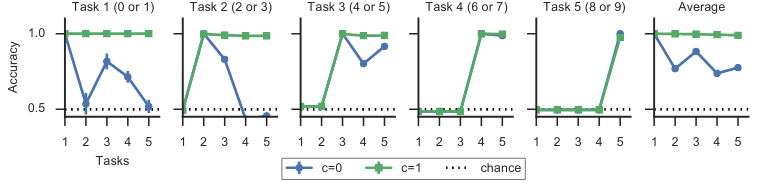
\includegraphics[width=\textwidth]{ML3}
	%\caption{Illustration of Catastrophic Forgetting \cite{zenke2017continual}}
\end{figure}
\end{frame}
\begin{frame}{Permuted MNIST}
	\begin{columns}
		\begin{column}{0.5\textwidth}
			\begin{itemize}
			\item Randomly permute all MNIST pixels for a task
			\item Performance measured by correctness across all tasks
			\item<2-> Correlations of $\omega_k^\mu$ decrease across different tasks $\mu$: "Using different weights to learn new tasks"
		\end{itemize}
		\end{column}
		\begin{column}{0.5\textwidth}
			\begin{figure}
				
				\centering
				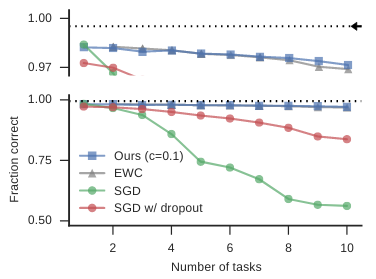
\includegraphics[width=\textwidth]{ML2}
				%\caption{Illustration of Catastrophic Forgetting \cite{zenke2017continual}}
			\end{figure}
		\end{column}
	\end{columns}

\end{frame}



\begin{frame}{Split CIFAR-10/CIFAR-100}
\begin{columns}
	\begin{column}{0.5\textwidth}
		\begin{itemize}
			\item First image classification on CIFAR-10, then 5 additional tasks  corresponding to 10 consecutive classes from CIFAR-100
			\item<2-> Better validation accuracy than networks trained on single task only: Less prone to overfitting
		\end{itemize}
	\end{column}
	\begin{column}{0.5\textwidth}
		\begin{figure}
			
			\centering
			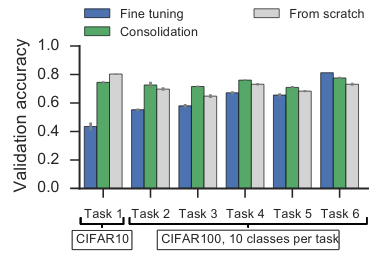
\includegraphics[width=\textwidth]{ML4}
			%\caption{Illustration of Catastrophic Forgetting \cite{zenke2017continual}}
		\end{figure}
	\end{column}
\end{columns}

\end{frame}

\begin{frame}{Discussion}
	\begin{itemize}
		\item Penalising changes to most important synapses can alleviate catastrophic forgetting
		\item<2-> EWC:
		\begin{itemize}
			 \item<2-> Offline, point estimate of posterior probability
			 \item<2-> Computing diagonal of Fisher has linear complexity in number of data points
		\end{itemize}
	\item<3-> Synaptic Intelligence
	\begin{itemize}
		\item<3-> Online estimate over entire learning trajectory
		\item<3-> Doesn't scale naturally to multiple tasks
	\end{itemize}
	\end{itemize}
\end{frame}
\begin{frame}{Outlook and Questions}
\begin{itemize}
	\item<1-> To what extent does this help to decrease the number of examples needed for learning new tasks?
	\item<2-> Fixing the hyperparameters $\lambda,c$ is quite expensive. Can we adaptively learn or predict them based on a priori knowledge about new task?
	\item<3-> Can we cluster important weights and use other sparsity regularisation strategies such as group Lasso?
\end{itemize}
\end{frame}

\begin{frame}
\begin{quote}
	\textcolor{oxfordblue}{In addition to adding depth to our networks, we may need to add intelligence to our synapses.}
\end{quote}
\end{frame}


\begin{frame}{References}

\bibliography{References}
\end{frame}
\end{document}

